%!Tex Root=**/main.tex
\mode<presentation>{\subsection{LangSplat}}
\mode<article>{\section{LangSplat}}

\begin{frame}<article>[c]
	\mode<all>{\Frametitle{Overview}}% Customized Title
    \mode<article>{Figure~\ref{fig:langsplat-overview} is the tagged framework of~\autocite{qinLangSplat3DLanguage2023}.}
	\begin{figure}[htbp]
		\centering
		\begin{annotatedFigureEnv}
			{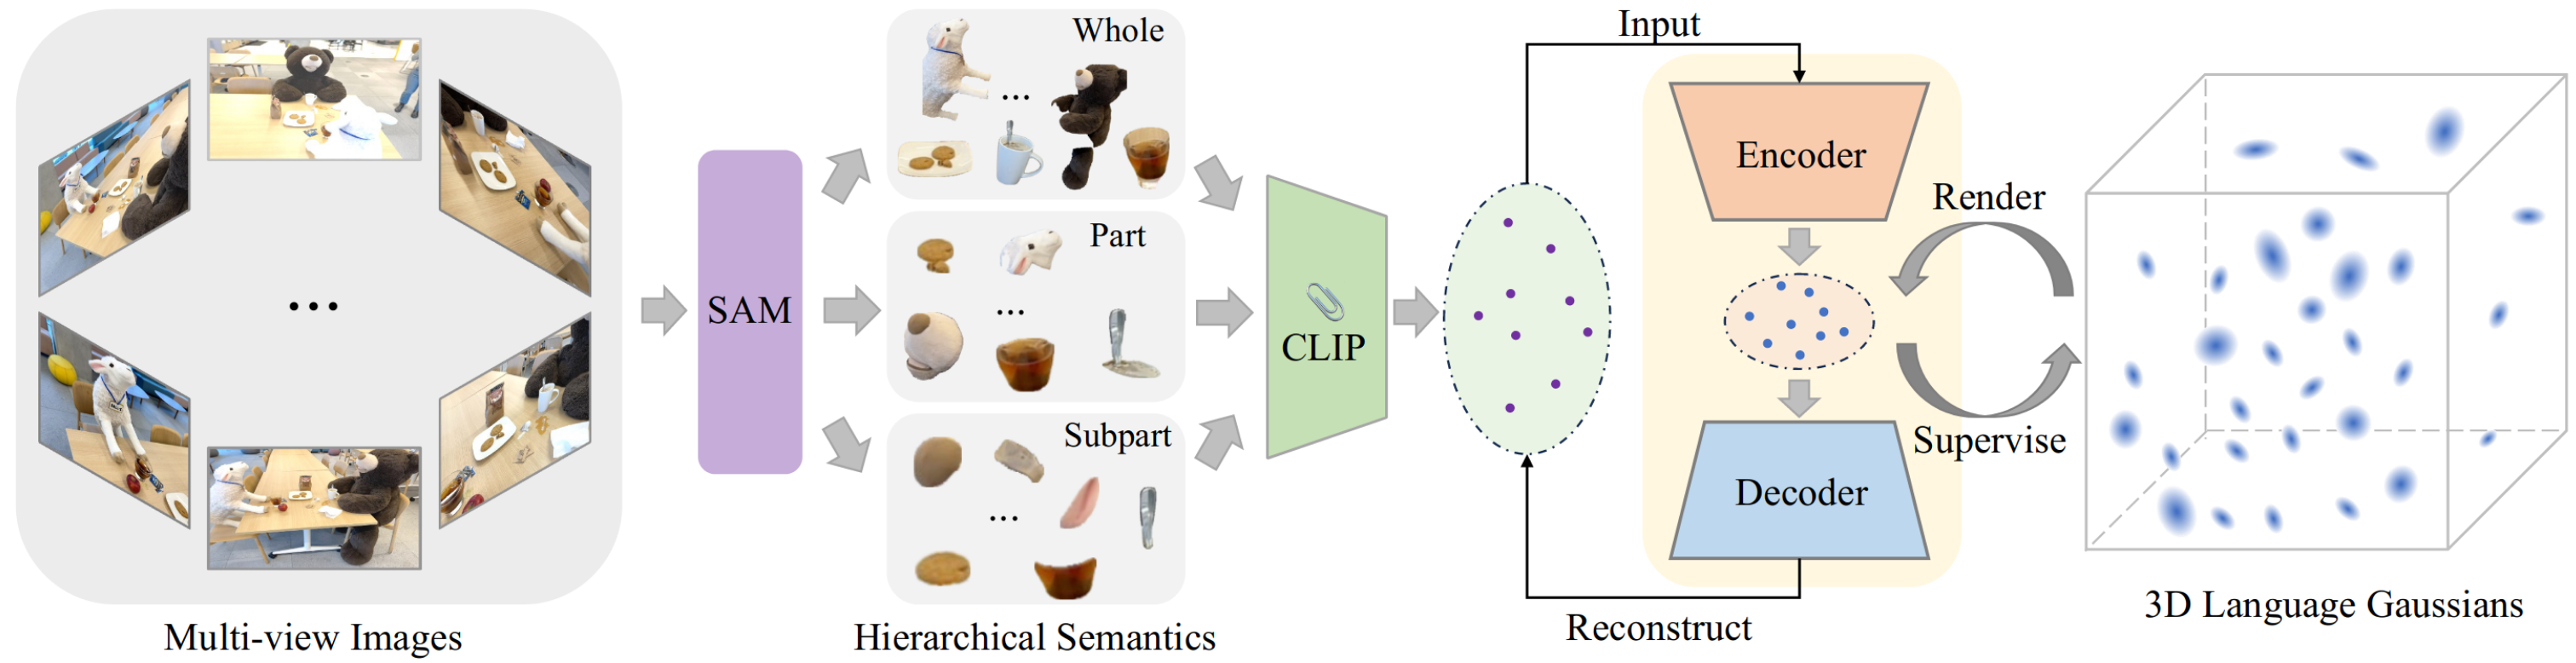
\includegraphics[width=0.8\linewidth]{langsplat-overview.png}}
			\annotatedFigure{0.25,0}{0.55,1}{1}{0.25,0}
			\annotatedFigure{0.55,0}{0.82,1}{2}{0.55,0}
		\end{annotatedFigureEnv}
		\vspace*{0.5ex}
        \caption{Overview of LangSplat}\label{fig:langsplat-overview}
	\end{figure}
	\begin{block}{Key Insights}
		\begin{enumerate}
			\item \alert{Accuracy:} SAM outputs to enhance CLIP features.
			      \begin{itemize}
				      \item \alert{CLIP:} image-aligned training leads to ``point-ambiguity''.
				      \item \alert{SAM:} pixel-aligned \& object-centered \& multi-granularity.
			      \end{itemize}
			\item \alert{Efficiency:} an \alert{auto-encoder} to compress latent features.
			      \begin{itemize}
				      \item More complexity and better compression, compared with ``speed-up module'' in Feature 3DGS~\autocite{zhouFeature3DGSSupercharging2024apr}.
			      \end{itemize}
		\end{enumerate}
	\end{block}
	\mode<presentation>{\blfootnote{\href{http://arxiv.org/abs/2312.16084}{(CVPR Highlight, 2024) LangSplat: 3D Language Gaussian Splatting}}}
\end{frame}

\begin{frame}<presentation>
	\Frametitle{Overview}
	\mode<presentation>{\blfootnote{\href{http://arxiv.org/abs/2312.16084}{(CVPR Highlight, 2024) LangSplat: 3D Language Gaussian Splatting}}}
	\begin{figure}[htbp]
		\centering
		\begin{annotatedFigureEnv}
			{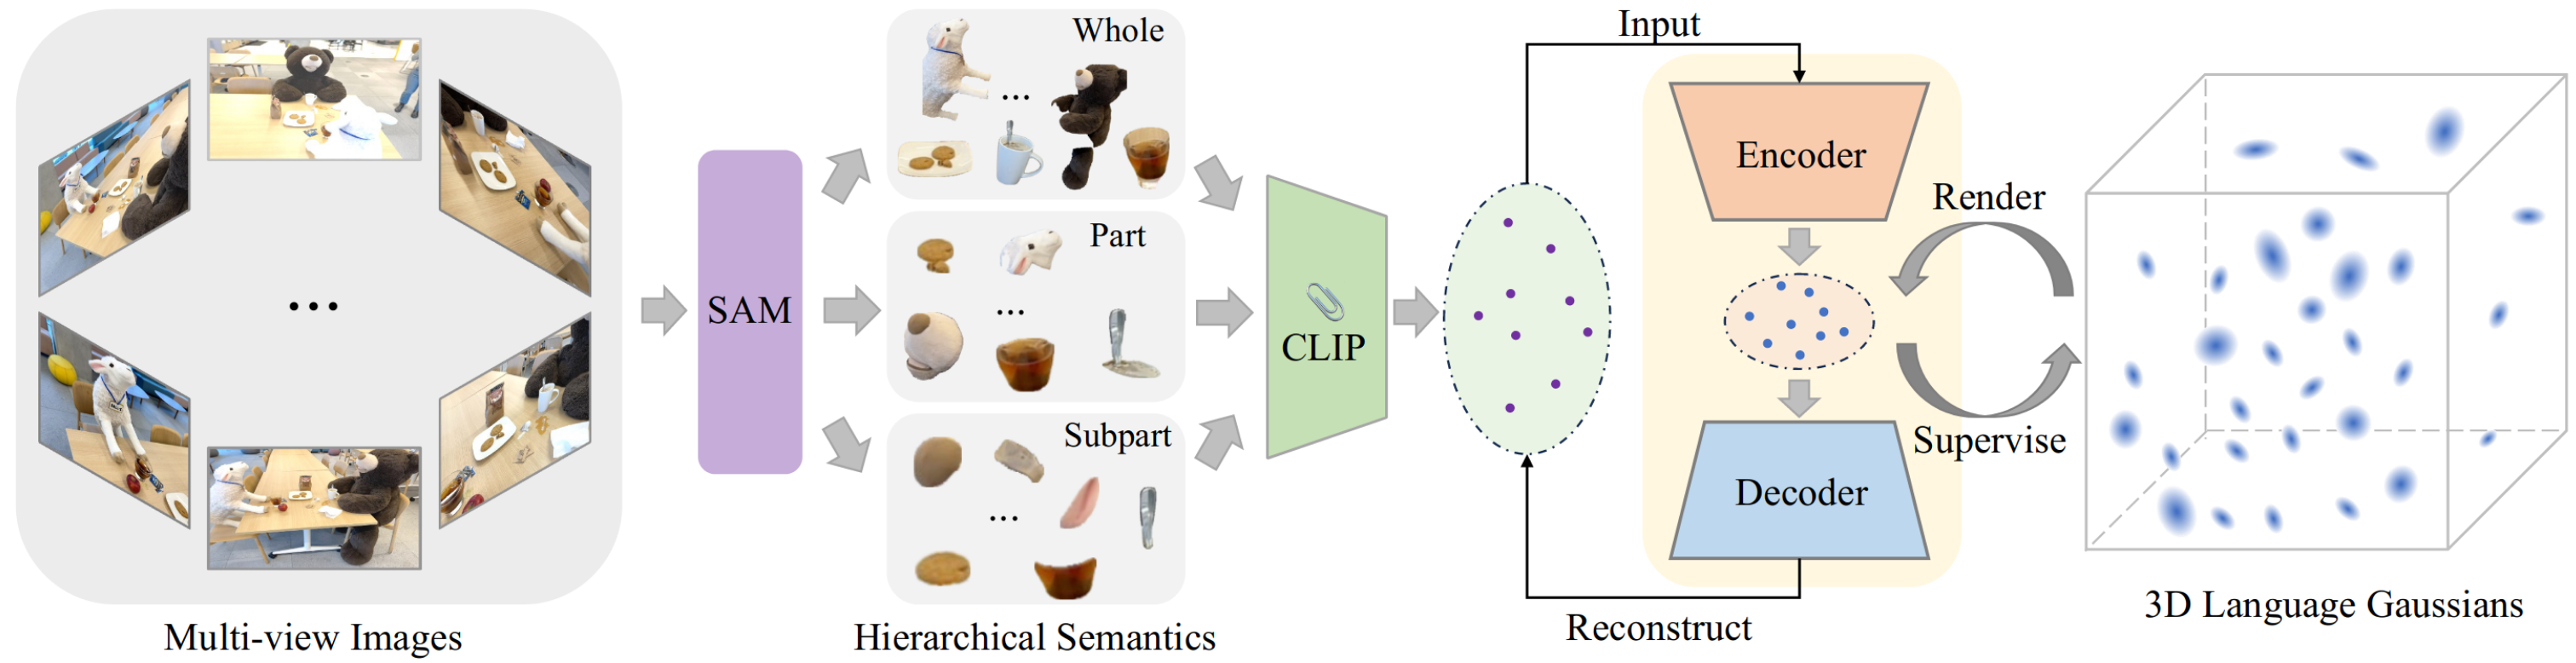
\includegraphics[width=0.8\linewidth]{langsplat-overview.png}}
			\annotatedFigure{0.25,0}{0.55,1}{1}{0.25,0}
			\mode<article>{\annotatedFigure{0.55,0}{0.82,1}{2}{0.55,0}}
		\end{annotatedFigureEnv}
		\caption{Overview of LangSplat}
	\end{figure}
	\mode<presentation>{\vspace*{\fill}}
	\begin{enumerate}[<+(1)->]
		\setlength{\itemsep}{1.5ex}
		\item \alert<.(1)>{Accuracy:} SAM outputs to enhance CLIP features.
		      \mode<presentation>{\vspace*{1.5ex}}
		      \begin{itemize}
			      \mode<presentation>{\setlength{\itemsep}{1.5ex}}
			      \item \alert<.(1)>{CLIP:} image-aligned training leads to ``point-ambiguity''.
			      \item \alert<.(1)>{SAM:} pixel-aligned \& object-centered \& multi-granularity.
		      \end{itemize}
	\end{enumerate}
\end{frame}

\begin{frame}<presentation>
	\mode<presentation>{\Frametitle{Overview}}
	\mode<presentation>{\blfootnote{\href{http://arxiv.org/abs/2312.16084}{(CVPR Highlight, 2024) LangSplat: 3D Language Gaussian Splatting}}}
	\mode<presentation>{
		\begin{figure}[htbp]
			\centering
			\begin{annotatedFigureEnv}
				{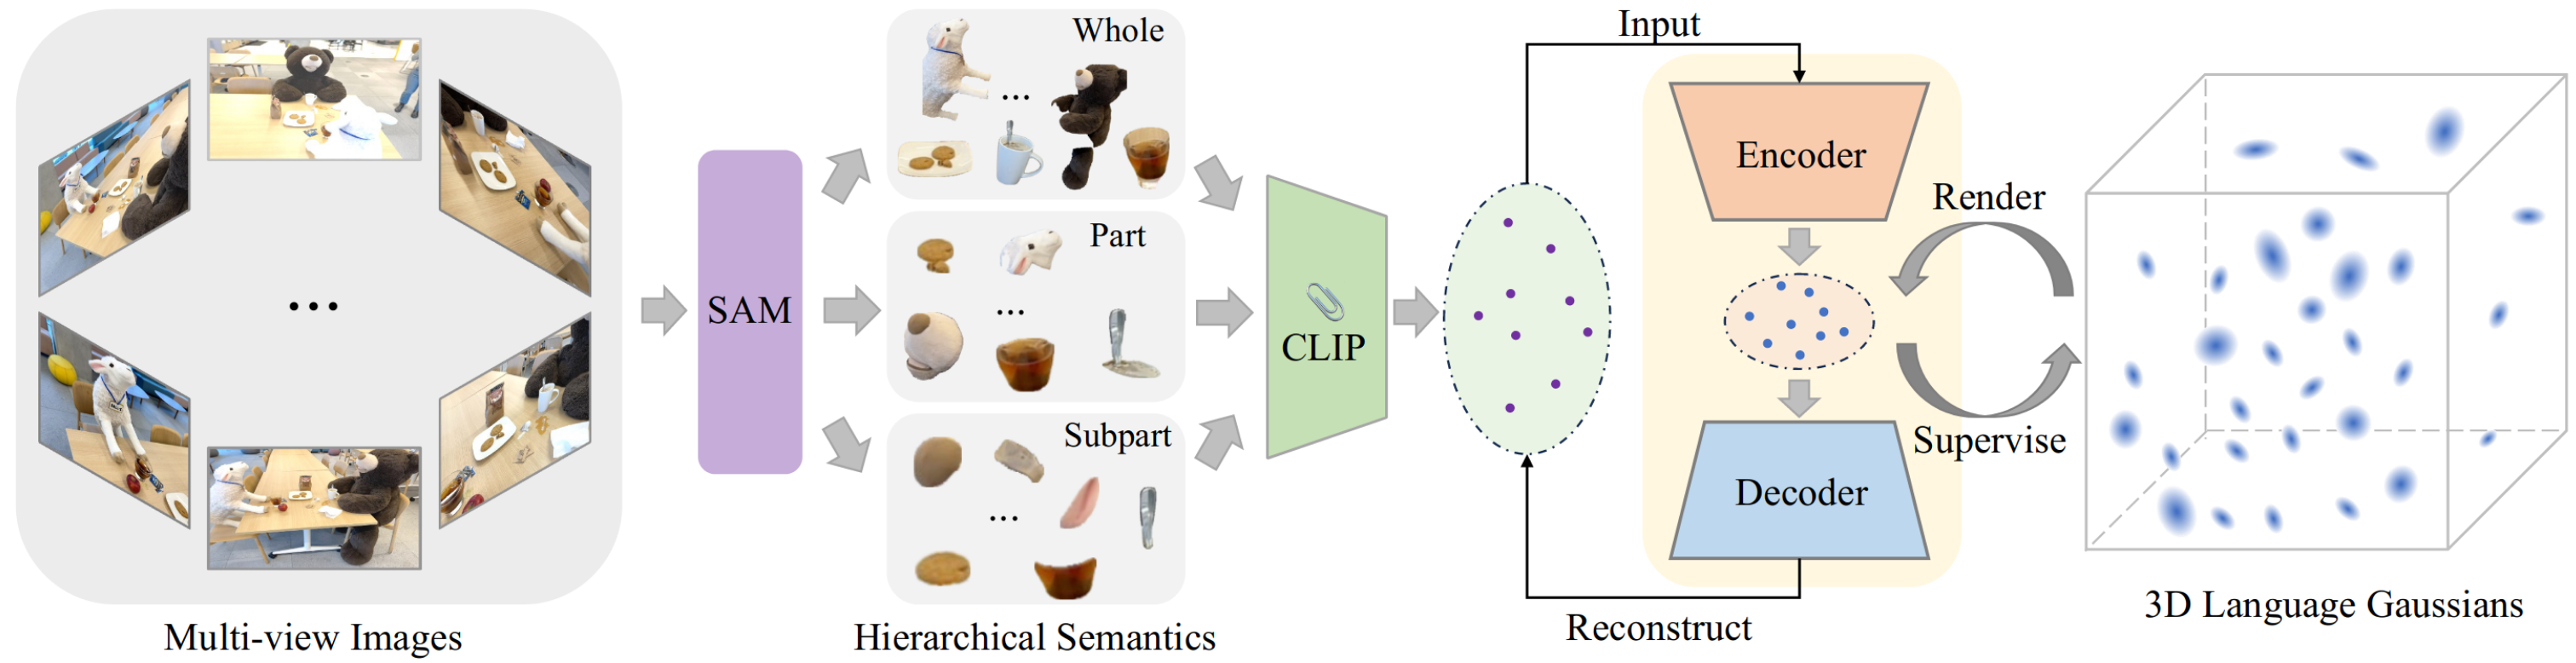
\includegraphics[width=0.8\linewidth]{langsplat-overview.png}}
				\annotatedFigure{0.55,0}{0.82,1}{2}{0.55,0}
			\end{annotatedFigureEnv}
			\addtocounter{figure}{-1}
			\caption{Overview of LangSplat}
		\end{figure}
		\mode<presentation>{\vspace*{\fill}}
	}
	\begin{enumerate}[<+->]
		\mode<presentation>{\setlength{\itemsep}{1.5ex}}
		\setcounter{enumi}{1}
		\item \alert<.>{Efficiency:} an \alert<.>{auto-encoder} to compress latent features.
		      \mode<presentation>{\vspace*{1.5ex}}
		      \begin{itemize}
			      \mode<presentation>{\setlength{\itemsep}{1.5ex}}
			      \item More complexity and better compression,
			            \mode<presentation>{\vspace*{1.5ex}}
			            \par compared with ``speed-up module'' in Feature 3DGS~\autocite{zhouFeature3DGSSupercharging2024apr}.
		      \end{itemize}
	\end{enumerate}
	\blfootnote{In practice, the latent dimension is \(3\) in the auto-encoder.}
\end{frame}
